\section{Evaluation}
\label{sec:evalution}

\subsection{Datasets and Experimental Setup}

%We use the following real-world datasets to test our proposed approach \mname{}, of discovering novel intents from unlabeled data and linking together mutually related intents: (i) SNIPS NLU benchmark~\cite{coucke2018} created by the company \textit{snips.ai}, (ii) ATIS NLU benchmark~\cite{dahl1994} from the flight reservation domain, (iii) Facebook semantic parsing dataset~\cite{gupta2018semantic}, and (iv) Internal NLU data\footnotemark from a commercial voice assistant. Statistics of these datasets are shown in Table~\ref{tab:stats}. 
We test \mname{} on the real-world datasets 
of SNIPS~\cite{coucke2018}%created by the company \textit{snips.ai}
, ATIS~\cite{dahl1994}%from the flight reservation domain
, Facebook's task-oriented semantic parsing (FTOP) data~\cite{gupta2018semantic}, and 
Internal NLU Data\footnotemark from a commercial voice assistant. 
For evaluation on SNIPS, ATIS and the Internal data, we completely remove all utterances associated with certain random sets of intents and domains from the training and validation sets, detailed in Table~\ref{tab:removed}. The FTOP dataset has intent types labeled as `unsupported', so we simply remove all utterances belonging to these intents while training \mname{}. Treating these removed intent and domain categories as novel (unseen), we then assess the efficacy of \mname{} in discovering these intents and domains during the testing phase. 
ATIS dataset intents are about airline reservations and are relatively similar to each other, while the SNIPS dataset consists of relatively dissimilar intent types. 
Our empirical configurations therefore holistically exhibit the performance of \mname{} when the novel intents being discovered have varying degrees of similarity with each other (or with the existing `seen' intents). 


\smallskip

\noindent \textbf{Hyperparameters:} %We now outline the exact implementation details and various hyperparameter values used in our algorithms. 
We used the English uncased BERT-Base model~\cite{devlin2018bert} in all steps of \mname{}. It has $12$ transformer layers, $768$ hidden states, and $12$ self-attention heads. We kept the dropout probability at $0.1$ and used the Adam optimizer~\cite{kingma2014adam} with parameters $\beta_1= 0.9$ and $\beta_2= 0.999$. We used slanted triangular learning rates~\cite{howard2018universal} for BERT with the base learning rate at $2e^{-5}$, and warm-up proportion at $0.1$. We empirically set the batch size to $64$, and the number of training epochs to $8$ for detecting instances with novel intents, and $15$ for discovering the latent intent categories. %, and save the best model on the validation set for testing.
To learn pairwise distances between utterances for clustering, we set $\alpha$ = $\beta$ = 1, and $m_1$ = $m_2$ = $m_3$ = 0.05. While discovering novel intent categories (Section~\ref{sec:stage2}), we used cosine similarity as the function `\textit{d(.)}' while computing $d(E(\bm{x}), E(\bm{x^p}))$, and euclidean distance as the function `\textit{f(.)}' while computing $f(Emb(\bm{x}), Emb(\bm{x^p}))$.
%Instead of saying 0, 0.5, 1: say i, j, k. Say in hyperparameters that we found 0,0.5,1 to work best for most datasets.
%m1=, m2=, m3=

\begin{comment}
The intents that we remove while training and aim to discover during evaluation for different datasets are:
\begin{enumerate}
\item SNIPS: Set 1: \textit{Weather, Restaurant}; and Set 2: \textit{AddToPlaylist, RateBook}.
\item ATIS: Set 1: \textit{airline, meal, airfare, day-name, distance}; and Set 2: \textit{ flight-time, flight-no, flight, ground-service, aircraft}. 
\item FTOP: Set 1:  \textit{unsupported, unsupported-event, unsupported-navigation, unintelligible}.
\item Internal NLU Dataset: we remove all intents present in the following domains: Set 1: \textit{Weather, Calendar, Todos}; Set 2: \textit{Sports, Local Search, Video, General Media, BookingsAndReservations}; Set 3: \textit{Recipe, Music, Shopping, Communication}; and Set 4: \textit{Global, Knowledge}.
\end{enumerate}
\end{comment}

\begin{table}[t]
\caption{Evaluating \mname{} on discovering novel intents and domains removed during training}
%\vspace{-0.6em}
\label{tab:removed} \centering
\small
\hskip-0.4cm\begin{tabularx}{1.03\linewidth}{L{0.15}|L{1.4}|L{0.17}|L{0.13}|L{0.15}}
\hline
\textbf{Dataset} & \textbf{Sets of intents removed from training data for evaluation} & \textbf{\# of data samples} & \textbf{Vocab size} & \textbf{Avg. text len.}  \\
\hline
SNIPS & \textbf{Set 1}: \textit{Weather, Restaurant}; \textbf{Set 2}: \textit{AddToPlaylist, RateBook} & 13.8K & 10.9K & 9.05 \\
ATIS & \textbf{Set 1}: \textit{airline, meal, airfare, day-name, distance}; \textbf{Set 2}: \textit{ flight-time, flight-no, flight, aircraft, ground-service}  & 5.87K & 0.87K & 11.2  \\
FTOP & \textbf{Set 1}:  \textit{unsupported, unsupported-event, unsupported-navigation, unintelligible} & 44.78K & 16.69K  & 8.93  \\
Internal NLU Dataset & \textbf{Set 1}: \textit{Weather, Calendar, Todos}; \textbf{Set 2}: \textit{Bookings\&Reservations, Sports, Local Search, Video, General Media}; \textbf{Set 3}: \textit{Recipe, Music, Shopping, Communication}; \textbf{Set 4}: \textit{Global, Knowledge}  & 3.16M & 26.7K & 3.72 \\
\hline
\end{tabularx}
\end{table}


%domain information is not available for SNIPS/ATIS, we only use x, xi and x, xk.

\begin{comment}
\begin{table}[t]
\caption{Statistics of the datasets used in our experiments}
%\vspace{-0.6em}
\label{tab:stats} \centering
\small
\begin{tabularx}{\linewidth}{L{0.87}|L{0.23}|L{0.19}|L{0.35}|L{0.36}}
\hline
\textbf{Dataset} & \textbf{SNIPS} & \textbf{ATIS} & \textbf{FTOP} & \textbf{Internal Dataset} \\
\hline
\# of data samples & 13.8K & 5.87K & 44.78K & 3.16M \\
Vocabulary size & 10.9K & 0.87K & 16.69K & 26.7K \\
Avg. utterance length & 9.05 & 11.2 & 8.93 & 3.72 \\
\hline
\end{tabularx}
\end{table}
\end{comment}

\footnotetext{Customer utterances from a voice-powered virtual assistant, whose name we omit for the double-blind review purpose.}


\subsection{Baselines and Evaluation Metrics} 

%We compare the first step of our proposed approach of detecting utterances with novel intents \textbf{``\mname{} \textit{(multi unseen + DOC)}"} with the following baseline approaches in Table~\ref{tab:stage1}: 
%(i) \textbf{DOC}~\cite{shu2017doc}: an open-world classification approach with a 1-vs-rest sigmoid layer on top of a CNN. It tightens the sigmoid decision boundary by learning statistical class-specific confidence thresholds. (ii) \textbf{IntentCapsNet}~\cite{xia2018}: a zero-shot learning method that uses capsule neural networks to discover emerging intents. (iii) \textbf{LOF-LMCL}~\cite{lin2019deep}: it uses a local outlier detection method on top of a Bi-LSTM trained with a large margin cosine loss to distinguish between intents seen and unseen during training. (iv) \textbf{\mname{} \textit{(one unseen)}/\mname{} \textit{(one unseen + DOC)}}: variants of \mname{} that use a single unseen class while training our classification model, with and without the additional check employing the class-specific confidence thresholds per the DOC heuristic. (v) \textbf{\mname{} \textit{(multi unseen)}}: \mname{} with multiple unseen classes while training our classification model and without the DOC heuristic. 
%For evaluation, we use the standard classification metrics of accuracy and F1-score.


We designate the first step of our proposed approach of detecting utterances with novel intents as \textbf{``\mname{} \textit{(m-unseen + DOC)}"}, and compare it with the following state-of-the-art approaches in Table~\ref{tab:stage1}: 

\smallskip
\noindent \noindent (i) \textbf{DOC}~\cite{shu2017doc}: uses a CNN with a 1-vs-rest sigmoid layer on top. It tightens the sigmoid decision boundary by learning class-specific confidence thresholds to detect novel intents. 

\noindent (ii) \textbf{IntentCapsNet}~\cite{xia2018}: uses capsule neural networks in a zero shot setting to discover newly emerging intents. 

\noindent (iii) \textbf{LOF-LMCL}~\cite{lin2019deep}: uses local outlier detection on top of a Bi-LSTM trained with a large margin cosine loss to classify seen and unseen intents.% seen and unseen during training. 

\noindent (iv) \textbf{\mname{} \textit{(1-unseen)}/\mname{} \textit{(1-unseen + DOC)}}: variants of \mname{} using an \textit{(S+1)}-class classification model (Section~\ref{sec:stage1}), with and without the additional check %employing the class-specific confidence thresholds 
per the DOC heuristic. 

\noindent (v) \textbf{\mname{} \textit{(m-unseen)}}: \mname{}'s \textit{(S+1)}-th class split into $m$ novel classes, without the DOC heuristic. 

\smallskip

\begin{table*}[t]
\centering
\caption{F1-score of various approaches for detecting if an utterance contains a novel intent or not.} %Different Sets denoting different intents removed from the training set and appearing as novel intents in the test set.}\smallskip
%\resizebox{0.95\textwidth}{!}{ % If your table exceeds the column or page width, use this command to reduce it slightly
\begin{tabularx}{\linewidth}{L{0.87}|L{0.11}|L{0.11}|L{0.11}|L{0.11}|L{0.25}|L{0.11}|L{0.11}|L{0.11}|L{0.11}} \hline
  \textbf{Approach} & \multicolumn{2}{c|}{\textbf{SNIPS}} & \multicolumn{2}{c|}{\textbf{ATIS}} & \textbf{FTOP} & \multicolumn{4}{|c}{\textbf{Internal Dataset}}  \\\cline{2-10}
    &  \textbf{Set1}   & \textbf{Set2}  &  \textbf{Set1}  & \textbf{Set2}  &  \textbf{Set1}  &  \textbf{Set1}  & \textbf{Set2} & \textbf{Set3}  & \textbf{Set4}  \\%\cline{2-13}
    %&  FT:0.83  & S$\leftarrow$T  &  S$\rightarrow$T  & S$\leftarrow$T  &  S$\rightarrow$T  & S$\leftarrow$T &  S$\rightarrow$T  & S$\leftarrow$T &  S$\rightarrow$T  & S$\leftarrow$T &  S$\rightarrow$T  & S$\leftarrow$T \\ \hline
    \hline
  DOC~\cite{shu2017doc}  & 0.73 & 0.69 & 0.71 & 0.7 & 0.76 & 0.7 & 0.73 & 0.72 & 0.71 \\ 
  IntentCapsNet~\cite{xia2018} & 0.81 & 0.77 & 0.7 & 0.75 & 0.8 & 0.82 & 0.83 & 0.78 & 0.8 \\ 
  LOF-LMCL~\cite{lin2019deep} & 0.79 & 0.73 & 0.68 & 0.74 & 0.78 & 0.84 & 0.8 & 0.82 & 0.81\\ 
  \mname{} \textit{(1-unseen)} & 0.76 & 0.73 & 0.68 & 0.72 & 0.78 & 0.77 & 0.75 & 0.79 & 0.8 \\ 
  \mname{} \textit{(1-unseen+DOC)} & 0.85 & 0.81 & 0.73 & 0.8 & 0.87 & 0.86 & 0.87 & 0.88 & 0.86\\ 
  \mname{} \textit{(m-unseen)} & 0.78 & 0.75 & 0.7 & 0.75 & 0.8 & 0.8 & 0.8 & 0.82 & 0.84 \\ 
  \mname{} \textit{(m-unseen+DOC)} & \textbf{0.9} & \textbf{0.87} & \textbf{0.78} & \textbf{0.84} & \textbf{0.9} & \textbf{0.9} & \textbf{0.92} & \textbf{0.9} & \textbf{0.9} \\ 
\hline
\end{tabularx}
%}
\label{tab:stage1}
\end{table*}


\begin{table*}[t]
\centering
\caption{Discovering the latent intent types for utterances with novel intents. `\#int.' shows the number of discovered intents, `GT' denotes the true number of intents, and `Pur.' denotes cluster purity.}\smallskip
%\resizebox{0.95\textwidth}{!}{ % If your table exceeds the column or page width, use this command to reduce it slightly
\begin{tabularx}{1.02\linewidth}{L{0.66}|L{0.12}|L{0.11}|L{0.12}|L{0.09}|L{0.12}|L{0.11}|L{0.12}|L{0.09}|L{0.12}|L{0.11}|L{0.12}|L{0.08}} \hline
  \textbf{Approach} & \multicolumn{4}{c|}{\textbf{SNIPS Set 1 (GT = 2)}} & \multicolumn{4}{c|}{\textbf{SNIPS Set 2 (GT = 2)}} & \multicolumn{4}{|c}{\textbf{FTOP Set 1 (GT = 4)}}  \\\cline{2-13}
    &  \footnotesize{\bf \#int.} & \textbf{NMI}  &  \textbf{Pur.}   &  \textbf{F1} &  \footnotesize{\bf \#int.} & \textbf{NMI}  &  \textbf{Pur.} &  \textbf{F1} &  \footnotesize{\bf \#int.} & \textbf{NMI}  &  \textbf{Pur.}   &  \textbf{F1}
    \\%\cline{2-13}
    \hline
  \mname{} \textit{(clf+hier)} & \textbf{3} & 0.78 & 0.9 & 0.76 & \textbf{3} & 0.7 & 0.8 & 0.69 & 24 & 0.4 & 0.56 & 0.38\\ 
  \mname{} \textit{(triplet+hier)} & 4 & 0.71 & 0.81 & 0.69 & 5 & 0.65 & 0.76 & 0.66 & 48 & 0.36 & 0.51 & 0.35\\ 
  \mname{} \textit{(ProdLDA)} & NA & 0.71 & 0.84 & 0.72 & NA & 0.66 & 0.79 & 0.68 & NA & 0.42 & 0.53 & 0.38\\ 
  \mname{} \textit{(pair+RCC)} & \textbf{3} & 0.79 & 0.9 & 0.77 & \textbf{3} & 0.7 & 0.8 & 0.7 & 30 & \textbf{0.5} & \textbf{0.63} & 0.41\\ 
  \mname{} \textit{(pair+hier)} & \textbf{3} & \textbf{0.8} & \textbf{0.92} & \textbf{0.78} & \textbf{3} & \textbf{0.72} & \textbf{0.83} & \textbf{0.71} & \textbf{19} & 0.46 & 0.61 & \textbf{0.51}\\ 
\hline
\end{tabularx}
%}
\label{tab:stage21}
\end{table*}


\begin{table*}[t]
\centering
\caption{Discovering the actual, latent novel intents and novel domains of input utterances. For Internal Data Sets 1 and 2, the first two columns show the number of new intents (\#int.) and new domains (\#dom.) discovered respectively. `GT ($d$, $i$)' denotes the true number of domains $d$ and intents $i$.}\smallskip
%\resizebox{0.95\textwidth}{!}{ % If your table exceeds the column or page width, use this command to reduce it slightly
\begin{tabularx}{\linewidth}{L{0.65}|L{0.15}|L{0.17}|L{0.11}|L{0.14}|L{0.1}|L{0.16}|L{0.17}|L{0.11}|L{0.14}|L{0.1}} \hline
  \textbf{Approach} & \multicolumn{5}{c|}{\textbf{Internal Data Set 1 (GT = 3, 22)}} & \multicolumn{5}{|c}{\textbf{Internal Data Set 2 (GT = 5, 53)}}  \\\cline{2-11}
    &  \footnotesize{\bf \# int.} & \footnotesize{\bf \# dom.} & \textbf{NMI}  &  \textbf{Purity}   &  \textbf{F1} &  \footnotesize{\bf \# int.} & \footnotesize{\bf \# dom.} & \textbf{NMI}  &  \textbf{Purity} &  \textbf{F1}
    \\%\cline{2-13}
    \hline
  \mname{} \textit{(clf+hier)} & 108 & 35 & 0.53 & 0.69 & 0.48 & 178 & 71 & 0.41 & 0.64 & 0.36  \\ 
  \mname{} \textit{(triplet+hier)} & 206 & 51 & 0.52 & 0.63 & 0.41 & 205 & 65 & 0.33 & 0.61 & 0.31  \\ 
  \mname{} \textit{(ProdLDA)} & NA & NA & 0.56 & 0.7 & 0.55 & NA & NA & 0.4 & 0.69 & 0.42   \\ 
  \mname{} \textit{(pair+RCC)} & 91 & 40 & 0.55 & 0.73 & 0.52 & 188  & 57 & 0.5 & 0.74 & 0.5 \\ 
  \mname{} \textit{(pair+hier)} & \textbf{74} & \textbf{29} & \textbf{0.6} & \textbf{0.75} & \textbf{0.6} & \textbf{167} & \textbf{36}  & \textbf{0.57} & \textbf{0.75} & \textbf{0.55} \\ 
\hline
\end{tabularx}
%}
\label{tab:stage22}
\end{table*}


%For evaluating the next two steps of discovering the actual intent categories in the user utterances and linking the newly discovered intents into domains, we denote our proposed method as \textbf{``\mname{} \textit{(pairwise emb)}"}, i.e. using distances between embeddings learned via our pairwise training technique as input to hierarchical clustering. We compare it with the following approaches: (i) \textbf{\mname{} \textit{(clf emb)}}: uses the representation learned by the 2nd to last BERT layer of our classification model in Figure~\ref{fig:stage1}, as input to hierarchical clustering. (ii) \textbf{\mname{} \textit{(triplet emb)}}: uses embeddings trained with a triplet loss function consisting of utterance triplets $(x, x^-, x^+)$, as input to hierarchical clustering. $x^-$ and $x^+$ refer to utterances containing the same domain and intent, and different domain and intent as utterance $x$ respectively. (iii) \textbf{\mname{} \textit{(ProdLDA)}}: uses a neural topic modeling algorithm ProdLDA~\cite{srivastava2017autoencoding} in order to discover the novel intent categories in place of clustering. Since ProdLDA requires the number of topics as input, we give it the number of clusters output by ``\mname{} \textit{(pairwise emb)}". We denote the most likely topic for each utterance as its intent. (iv) \textbf{\mname{} \textit{(pairwise + RCC)}}: uses embeddings learned via our pairwise margin loss function as input to the Robust Continuous Clustering algorithm (RCC)~\cite{shah2017robust}, instead of hierarchical clustering. 


The first stage of discovering utterances with novel intents (Section~\ref{sec:stage1}) is evaluated using the standard F1-score metric. For evaluating the next two stages of discovering the actual intent categories in the user utterances and linking the newly discovered intents into domains (Sections~\ref{sec:stage2} and~\ref{sec:stage3}), we designate our proposed method as \textbf{``\mname{} \textit{(pair+hier})"}, i.e. using distances between embeddings learned via our pairwise margin loss function as input to hierarchical clustering. %We compare it with these baselines:
As per our knowledge, work in the literature only detects if text utterances contain novel intents or not, and does not identify the actual, latent intent categories in unlabeled text. Therefore, we compare \mname{} with its own variant baselines: %different variants of ADVIN in Tables 4 and 5. %We also experimented with a number of different clustering approaches (apart from hierarchical clustering), but did not include these results due to lack of space.

\smallskip

\noindent (i) \textbf{\mname{} \textit{(clf+hier)}}: uses the representation learned by the 2nd to last BERT layer of our classification model in Figure~\ref{fig:stage1}, as input to hierarchical clustering. 

\noindent (ii) \textbf{\mname{} \textit{(triplet+hier)}}: uses embeddings learned by a triplet network~\cite{schroff2015facenet} as input to hierarchical clustering. The inputs to the network are utterance triplets $(x, x^-, x^+)$. $x^-$ and $x^+$ contain the same domain and intent, and different domain and intent as utterance $x$ respectively. 

\noindent (iii)  \textbf{\mname{} \textit{(ProdLDA)}}: uses a neural topic modeling method ProdLDA~\cite{srivastava2017autoencoding} to discover novel intent categories, instead of clustering. %We denote the most likely topic for each utterance as its intent. 
ProdLDA requires the number of topics as input, so we give it the number of clusters output by ``\mname{} \textit{(pair+hier)}".

\noindent (iv) \textbf{\mname{} \textit{(pair+RCC)}}: uses embeddings learned via our pairwise loss function as input to the Robust Continuous Clustering algorithm (RCC)~\cite{shah2017robust}, instead of hierarchical clustering. 
\smallskip

Ground truth intent and domain labels are available for the various experimental data Sets we used for evaluation (Table~\ref{tab:removed}). We thus use the following standard clustering metrics to evaluate the novel intents and domains discovered: (i) Comparing the number of discovered intents and domains to the ground truth number. (ii) Normalized Mutual Information (NMI): a normalization of the mutual information by a generalized mean of the entropy of the ground truth and the entropy of the predicted cluster labels. %, to scale the result between 0 (no mutual information) and 1 (perfect correlation). 
(iii) Purity: the extent to which a cluster contains utterances with a single intent or domain. (iv) F1 score.

\subsection{Results}

\noindent \textbf{Baseline Comparison: } Table~\ref{tab:stage1} shows the F1-score of various approaches, on classifying an intent as novel or not on different datasets with different dataset configurations. We observe that our approach using an $(S+m)$-class classifier during training and the DOC heuristic, ``\mname{} \textit{(m-unseen+DOC)}", outperforms all baselines on all datasets by at least 6\% F1 score points. \mname{} also outperforms the zero shot IntentCapsNet model (that uses relevant information available beforehand about the new test intents to be discovered), without using any prior knowledge about the novel intents or domains.


Tables~\ref{tab:stage21} and~\ref{tab:stage22} show the performance of different approaches in discovering intent categories for the utterances containing novel intents as predicted in Table~\ref{tab:stage1}. We observe that our proposed approach ``(\mname{} + \textit{pair+hier})" using distances learned via our pairwise loss training method along with hierarchical clustering outperforms the rest of the baselines. The learned intent-clusters have a purity value more than 80\% for the SNIPS dataset. Purity decreases to $61\%$ for FTOP, primarily because semantically diverse utterances have been given the same ground truth intent label of \textit{`unsupported'} or \textit{`unsupported-event'}. The `NA' value for ``\mname{} \textit{(ProdLDA)}" in the column `\# int.' denotes that the \textit{ProdLDA} algorithm by design does not output the number of new intents discovered. It takes this as input in the form of the number of topics. We observe similar empirical trends as above on ATIS Sets 1 and 2, and Internal NLU Data Sets 3 and 4. In the interests of space, we do not present these results.

\begin{comment}
\begin{figure}[t]
\centering

\includegraphics[width=8.7cm,height=6cm]{Figures/tsne} % Reduce the figure size so that it is slightly narrower than the column. Don't use precise values for figure width.This setup will avoid overfull boxes. 
\caption{Visualizing embeddings learned by \mname{} for novel intents discovered within the \textit{`unsupported'} FTOP category.}
\label{fig:tsne}
\end{figure}
\end{comment}



Our technique discovers $1.5$-$4.5$ times more novel intents than present in the ground truth, as seen from the `\# int.' columns in Tables~\ref{tab:stage21} and~\ref{tab:stage22}. To investigate this further, we use t-SNE~\cite{maaten2008visualizing} to visualize the embeddings learned by training our proposed \mname{} method, for the utterances belonging to the \textit{`unsupported'} intent category of the FTOP dataset. In Figure~\ref{fig:tsne}, each color represents a different novel intent category discovered. We also show the most frequent utterance words present in each newly emergent intent. 
We observe that \textit{`Unsupported'} has been split up by \mname{} into $7$ finer-grained, semantically sensible novel intents. For instance, the utterances \textit{``What city has the most traffic in the US"} and \textit{``Family friendly bars near me"}, from the \textit{`unsupported'} intent category, have been separated by \mname{} into different intent categories.  Figure~\ref{fig:tsne} also explains the lower performance values in Table~\ref{tab:stage21} for the FTOP dataset. We thus find that \mname{} largely learns semantically appropriate, discriminative representations for the newly emerging intents (also echoed by our user study in Table~\ref{tab:user study}).


\begin{figure}
\begin{minipage}[c][7cm][t]{.5\textwidth}
  \vspace*{\fill}
  \centering
  {\label{fig:tsne}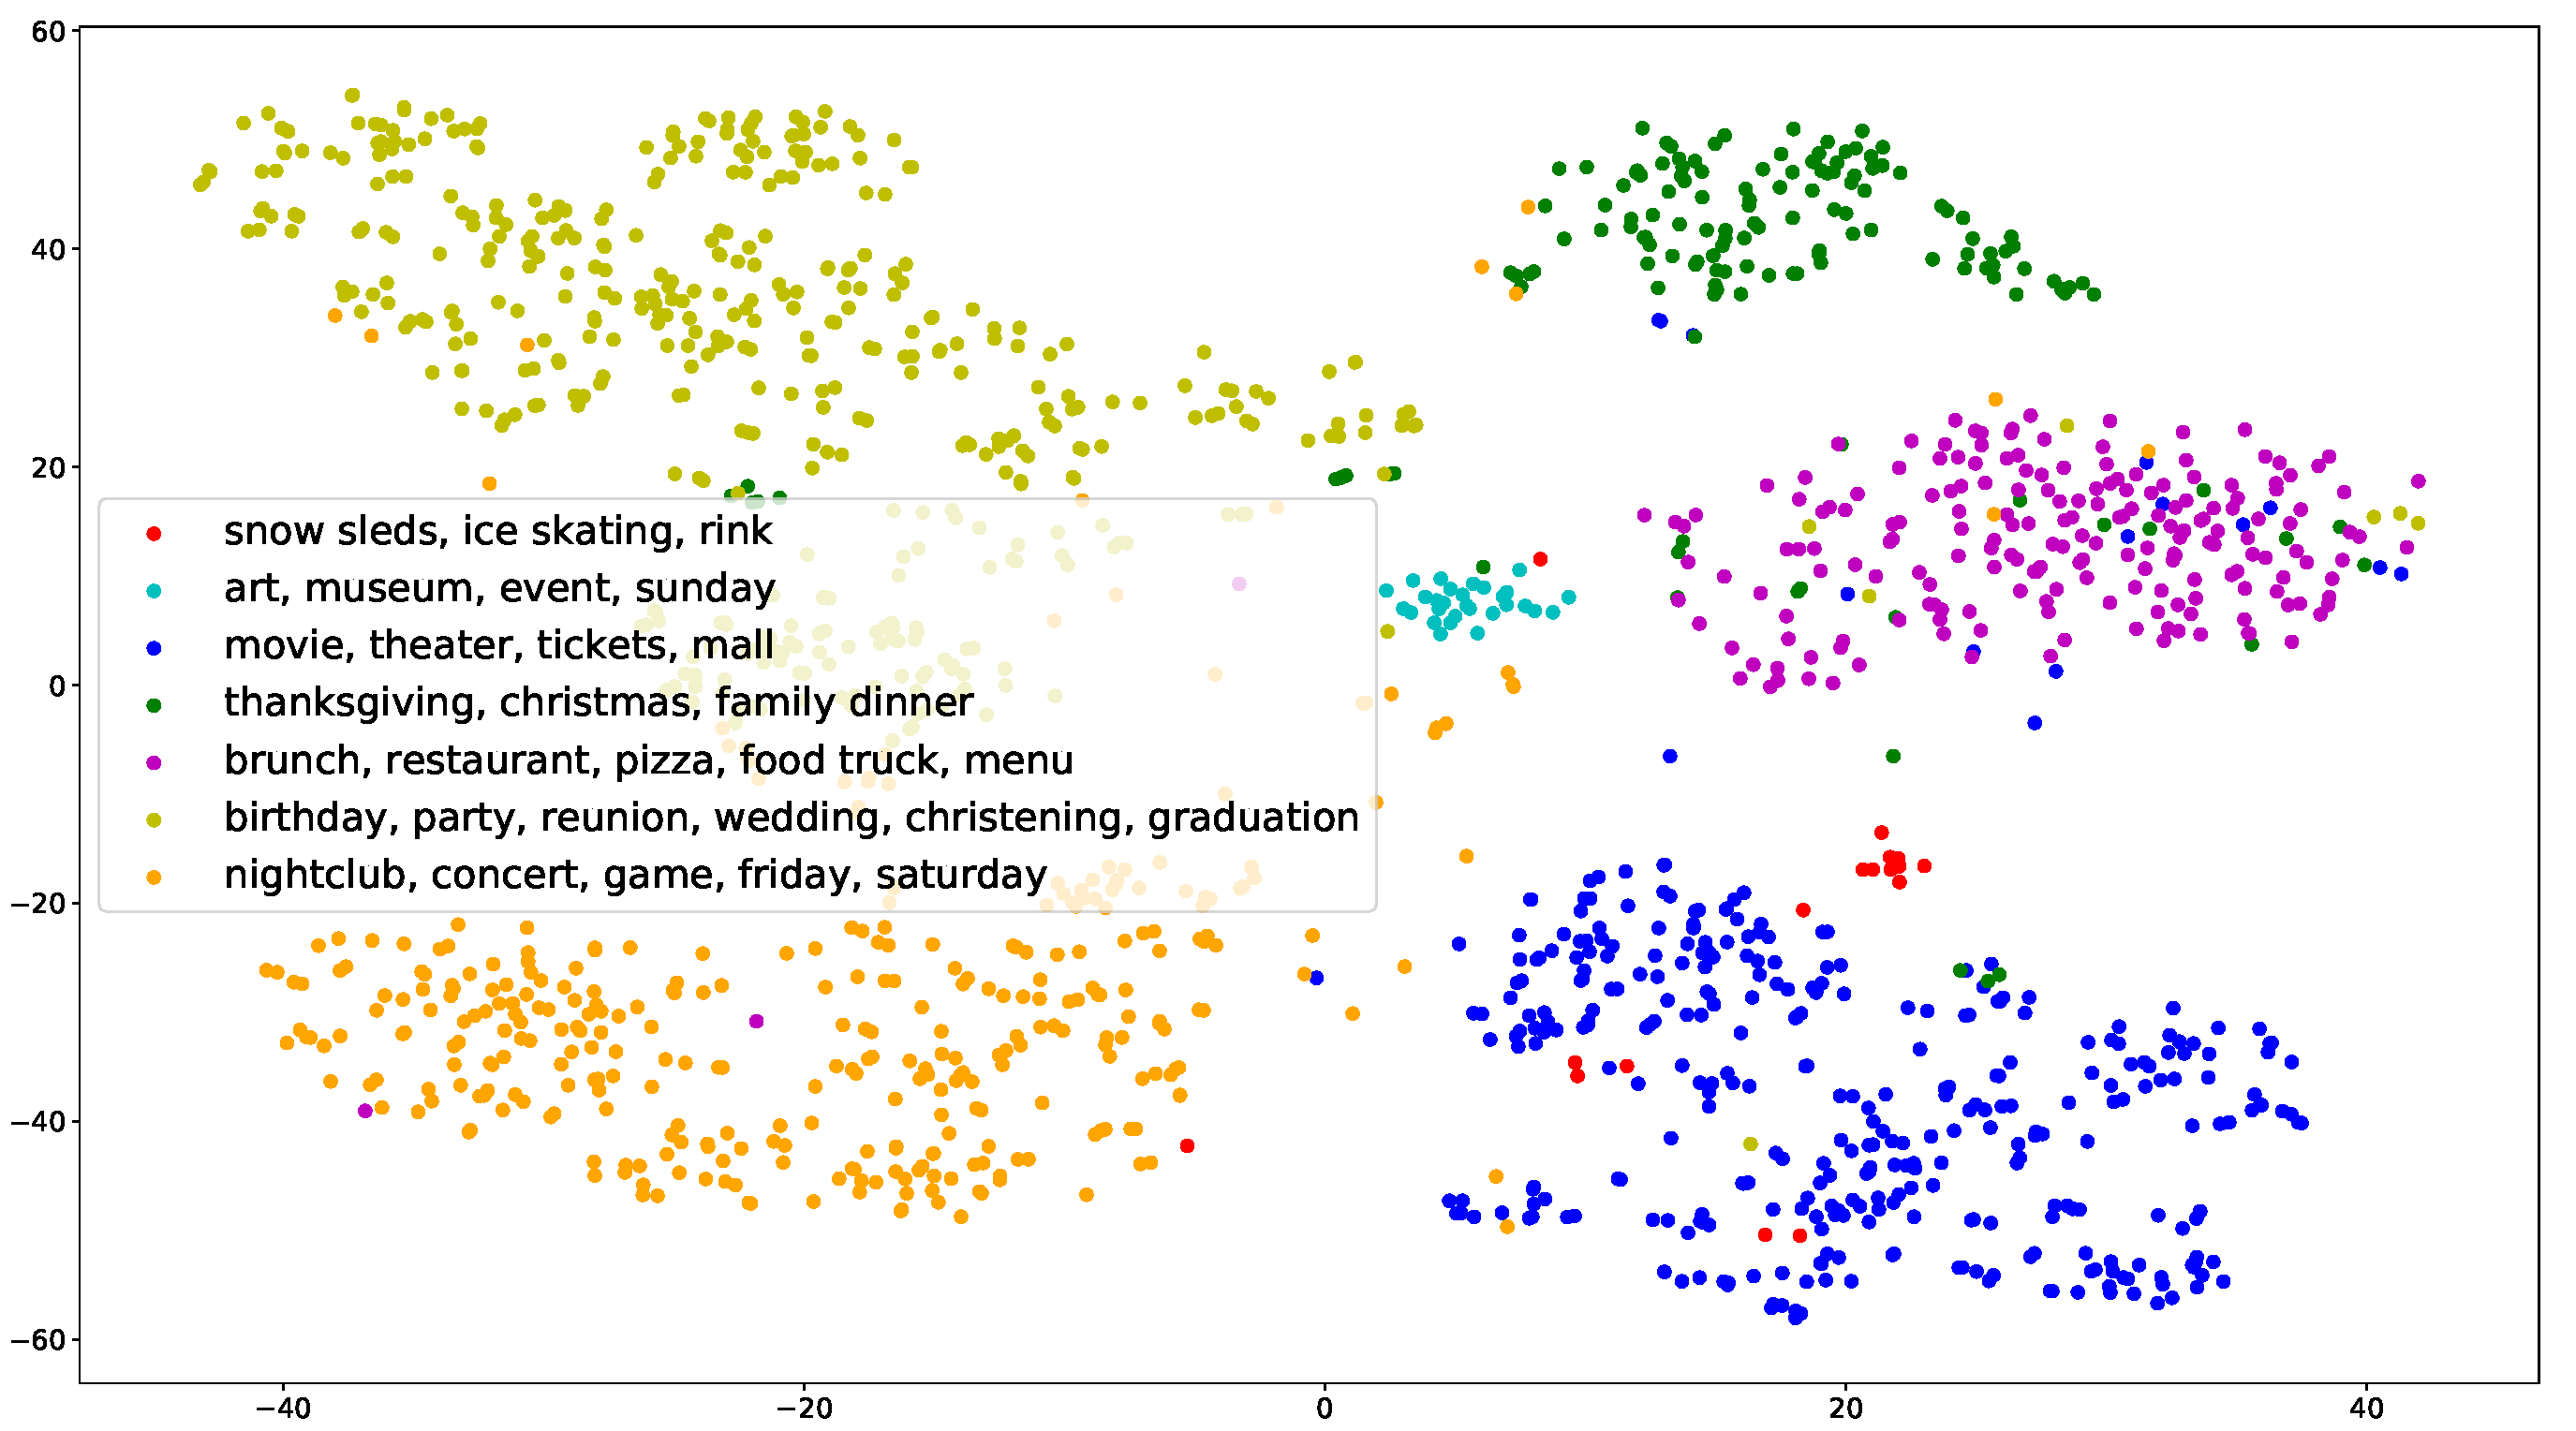
\includegraphics[width=8.6cm,height=6cm]{tsne}}
  \subcaption{}
\end{minipage}%
\begin{minipage}[c][7cm][t]{.5\textwidth}
  \vspace*{\fill}
  \centering
  {\label{fig:num_ood_intents}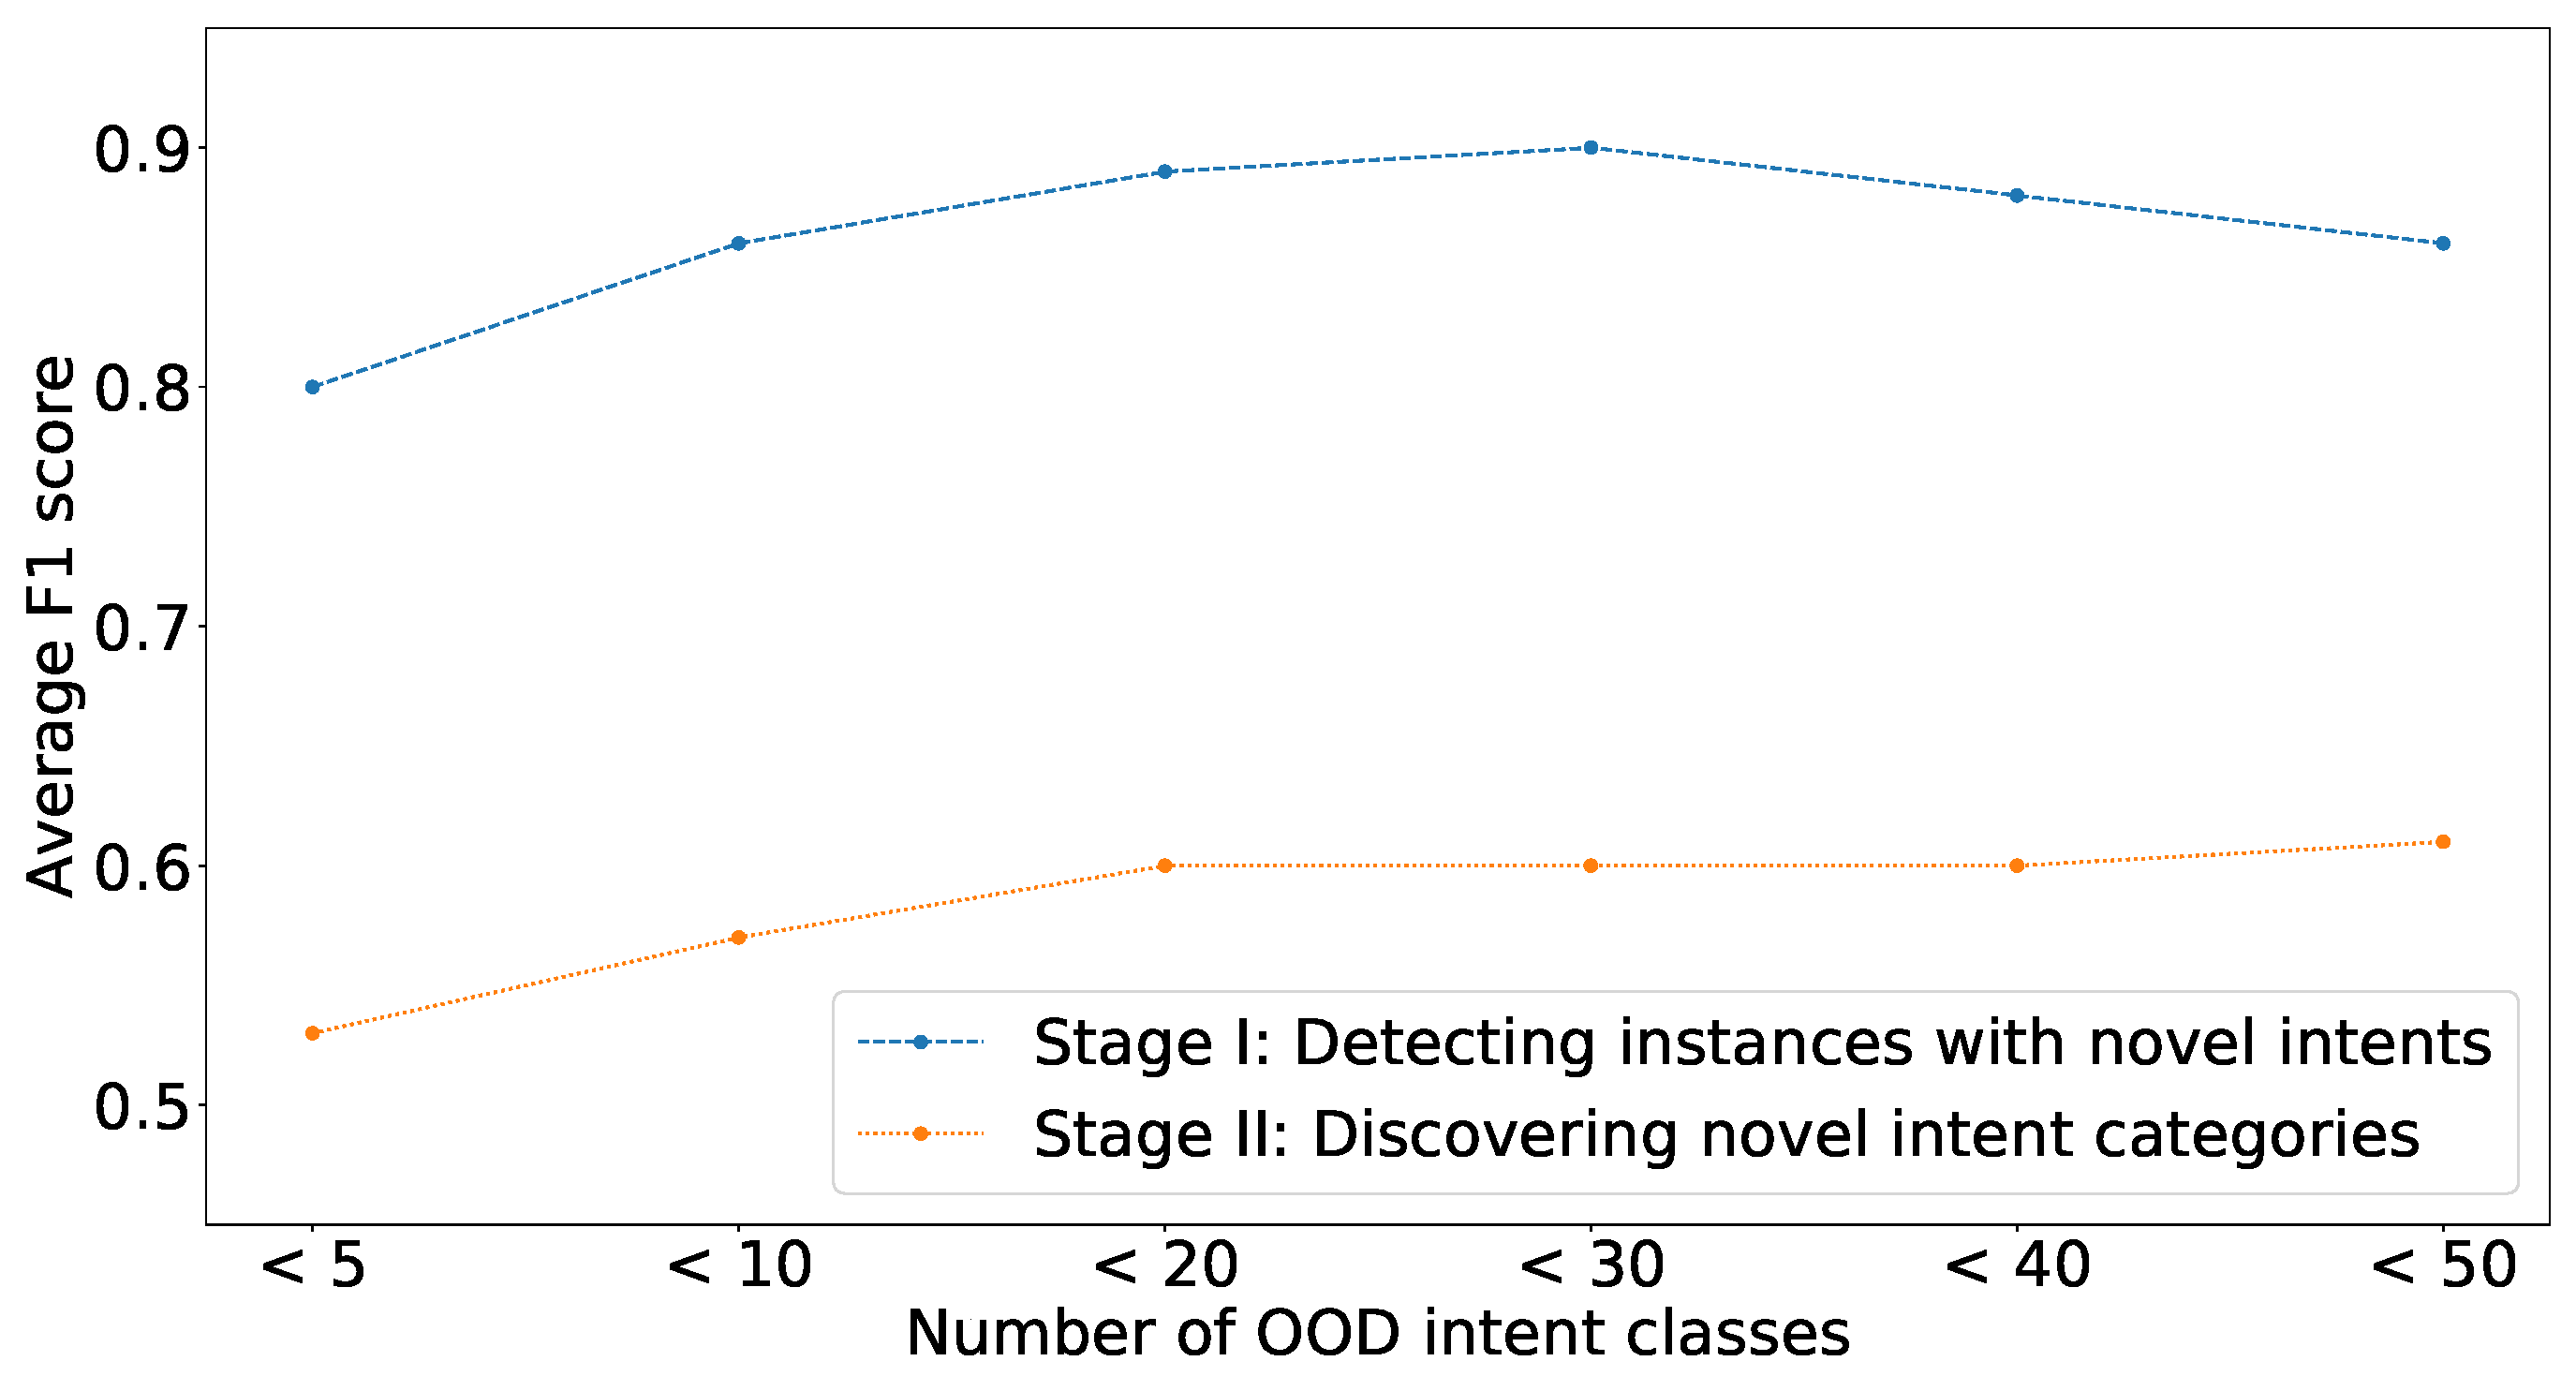
\includegraphics[width=6cm,height=2.8cm]{num_ood_intents_f1}}
  \subcaption{}
  \par\vfill
  {\label{fig:num_ood_intents}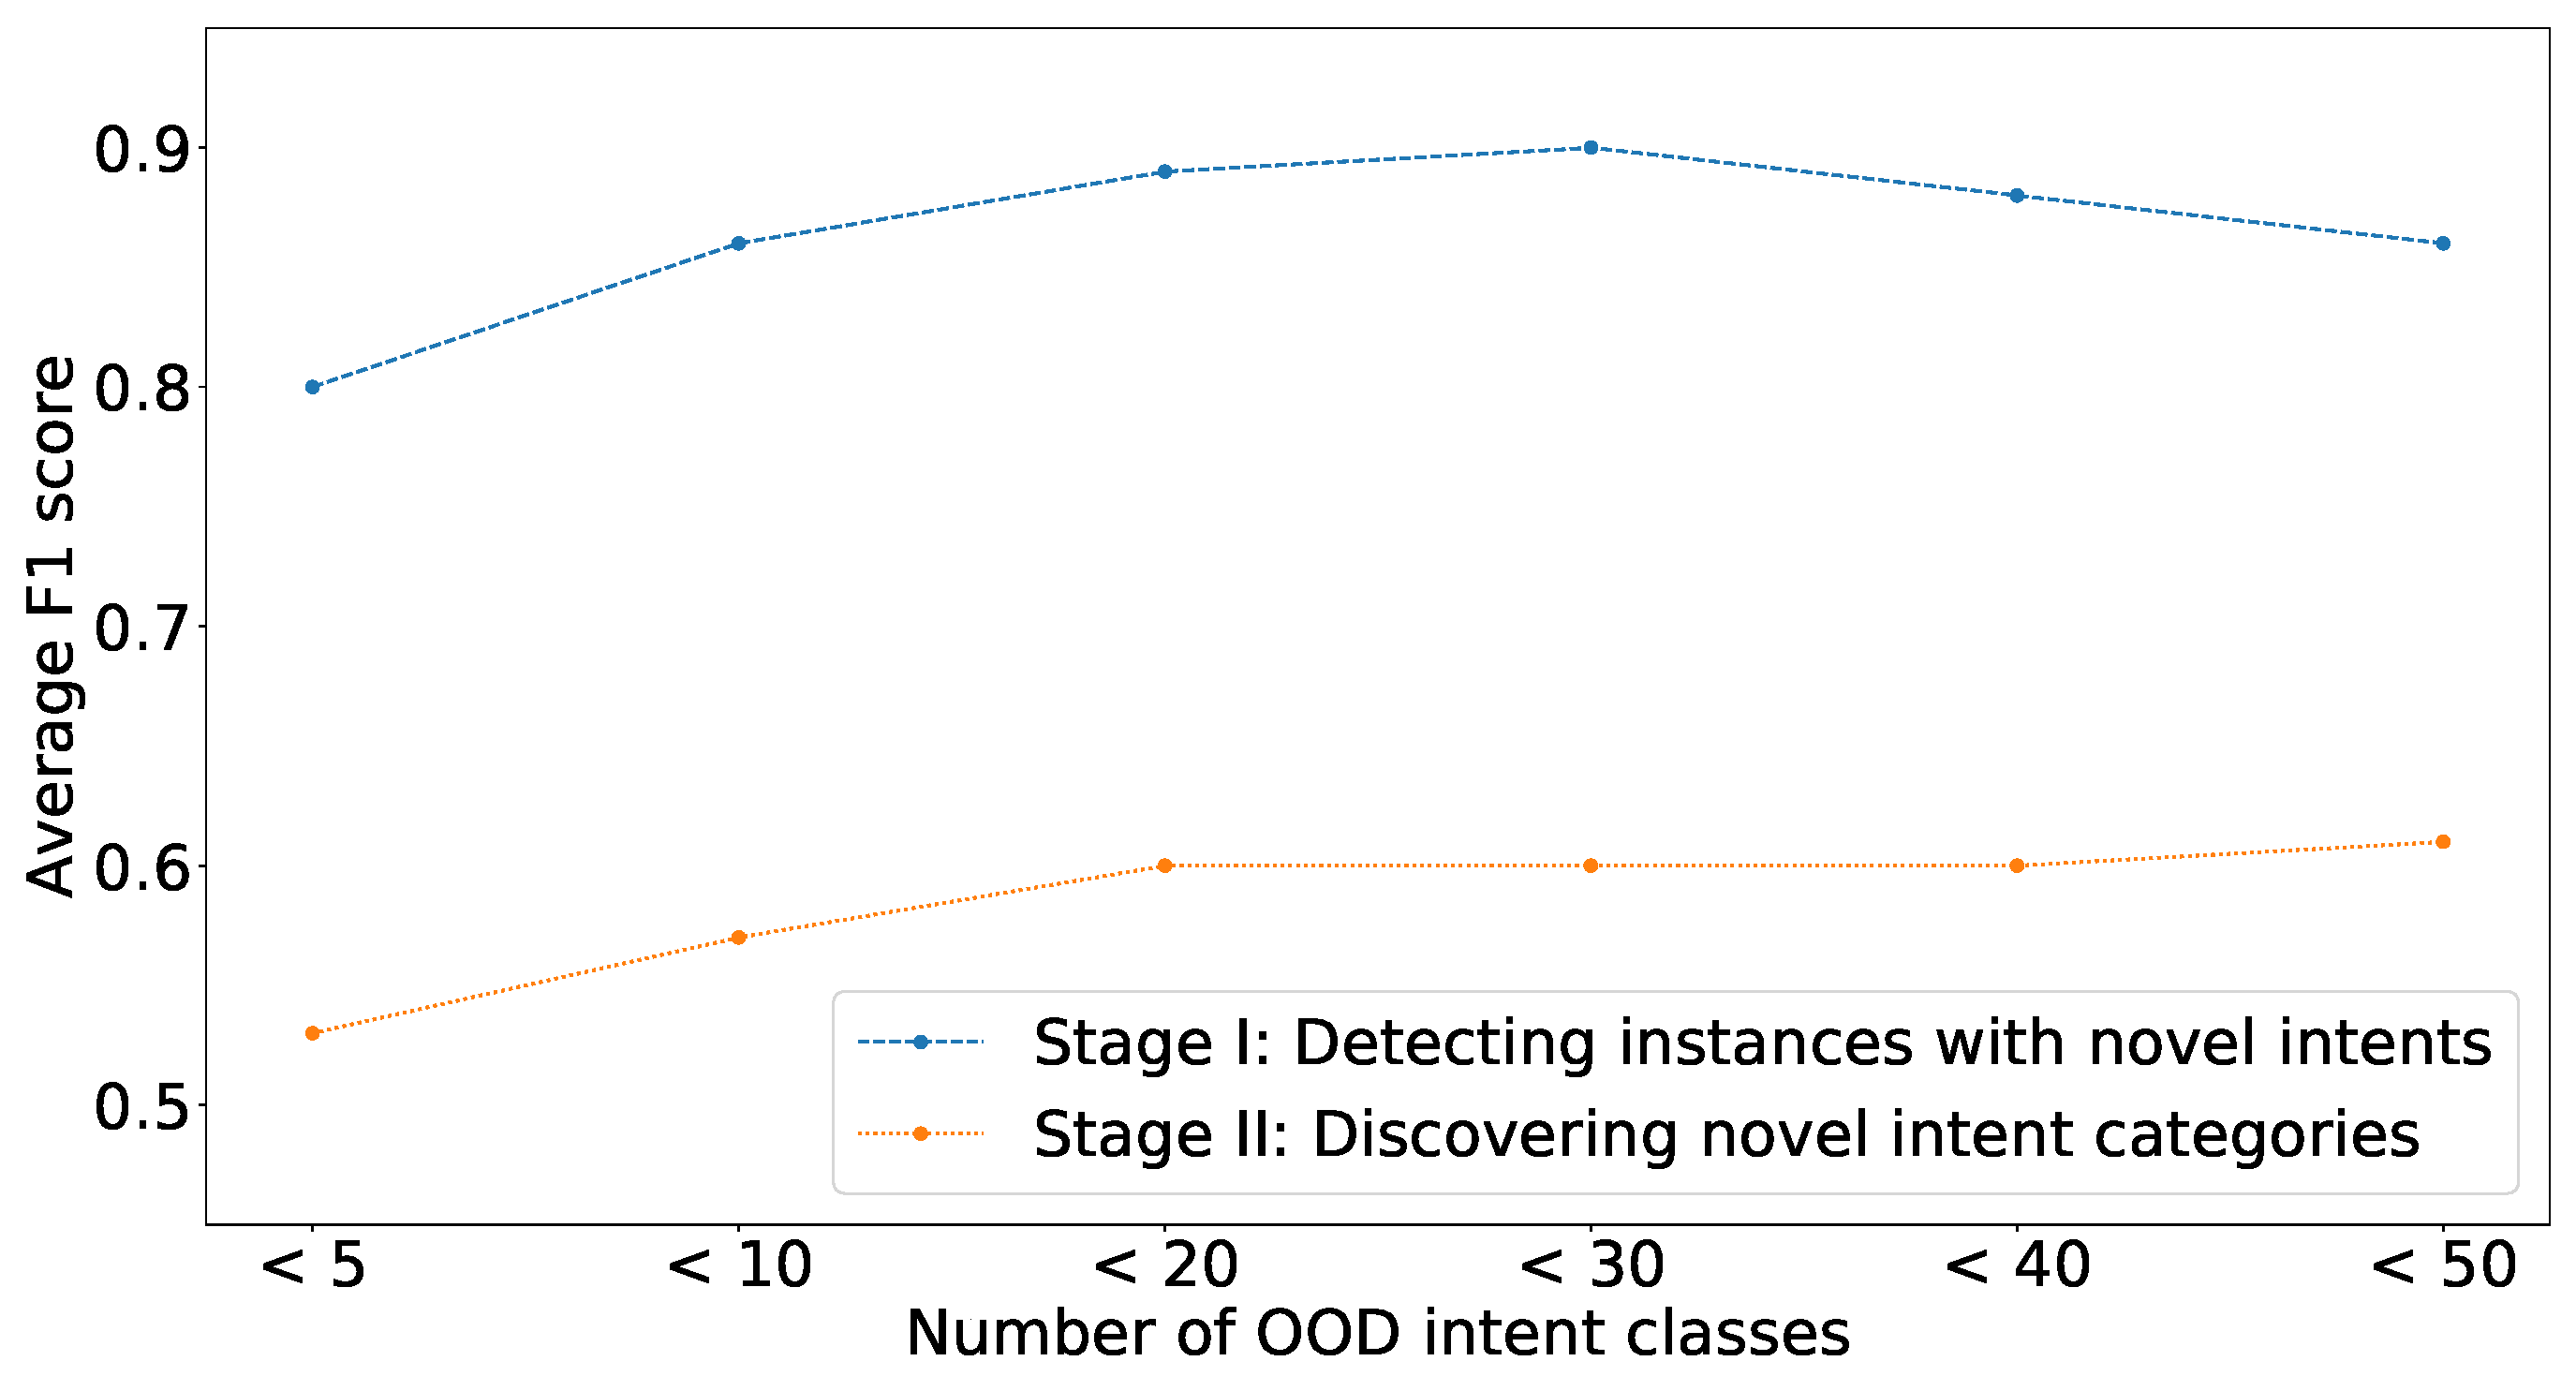
\includegraphics[width=6cm,height=2.8cm]{num_ood_intents_f1}}
  \subcaption{}
\end{minipage}
\caption{(a) Visualizing embeddings learned by \mname{} for novel intents discovered within the \textit{`unsupported'} FTOP category. The figure also shows the varying F1 score averaged across (b) number of OOD intent classes and (c) number of labeled OOD instances, given as training data for Stage I.}
\end{figure}


\begin{comment}
\begin{figure}
\centering
\sbox{\measurebox}{%
  \begin{minipage}[b]{.4\textwidth}
  \hspace{-1.5cm}
  \subfloat
    []
    {\label{fig:tsne}
\includegraphics[width=8.6cm,height=6cm]{Figures/tsne}}
  \end{minipage}}
\usebox{\measurebox}
\qquad
\begin{minipage}[b][\ht\measurebox][s]{.4\textwidth}
\centering
\subfloat
  []
  {\label{fig:num_ood_intents}
\includegraphics[width=6cm,height=2.8cm]{Figures/num_ood_intents_f1}}

\vfill

\subfloat
  []
  {\label{fig:num_ood_data}
\includegraphics[width=6cm,height=2.8cm]{Figures/num_ood_data_f1}}
\end{minipage}

\caption{(a) Visualizing embeddings learned by \mname{} for novel intents discovered within the \textit{`unsupported'} FTOP category. The figure also shows the varying F1 score averaged across (b) number of OOD intent classes and (c) number of labeled OOD instances, given as training data for Stage I.}
\end{figure}
\end{comment}


\begin{comment}
\begin{table}[H]
    \hskip-0.5cm\begin{minipage}{.1\linewidth}
      \centering
      \caption{F1-scores evaluating \mname{}'s prediction on unseen utterance pairs containing the same novel intent or not, w.r.t user study annotations. Parentheses show F1-scores using the dataset-provided annotations as ground truth.}
    \label{tab:user study}
      \begin{tabular}{c|c|c} \hline
  \textbf{Approach} & \textbf{FTOP} & \textbf{Internal} \\ \hline
  \mname{} \textit{(clf+hier)} & 0.66 (0.6) & 0.6 (0.68) \\ 
  \mname{} \textit{(triplet+hier)} & 0.6 (0.57) & 0.55 (0.61)  \\ 
  \mname{} \textit{(ProdLDA)} & 0.65 (0.56) & 0.54 (0.61)  \\ 
  \mname{}\textit{(pair+RCC)} & 0.64 (0.6) & 0.56 (0.64)  \\ 
  \mname{} \textit{(pair+hier)} & 0.7 (0.61) & 0.61 (0.71)  \\ 
\hline
\end{tabular}
%}
    \end{minipage}
    \hskip0.5cm\begin{minipage}{1.3\linewidth}
      \centering
      \caption{Performance of \mname{} of discovering intent categories within unlabeled utterances containing novel intents, on providing limited supervision as pairwise constraints. Parentheses show the results without providing supervision.}
    \label{tab:supervision}
      \begin{tabular}{c|c|c|c|c} \hline
  \textbf{Dataset} & \textbf{\# int.} & \textbf{NMI} & \textbf{Purity} & \textbf{F1}
    \\%\cline{2-13}
    \hline
  SNIPS S1 & 2 (3) & 0.82(2\%) & 0.94(2\%) & 0.85(7\%) \\ 
  ATIS S1 & 12(13) & 0.74(2\%) & 0.77(4\%) & 0.75(3\%)  \\ 
  FTOP & 17(19) & 0.5(4\%) & 0.64(3\%) & 0.54(3\%)  \\ 
  Internal 1 & 45(56) & 0.65(5\%) & 0.75(4\%)  &  0.65(3\%) \\ 
  Internal 2 & 82(92) & 0.58(4\%) & 0.7(1\%)  & 0.61(3\%)  \\ 
  Internal 3 & 90(131) & 0.6(4\%) & 0.75(3\%)  & 0.6(3\%)  \\ 
  Internal 4 & 127(141) & 0.62(3\%) & 0.69(2\%)  &  0.61(2\%) \\ 
\hline
\end{tabular}
    \end{minipage}
  \end{table}
\end{comment}


%\begin{comment}
\begin{table}[t]
\centering
\caption{Evaluating \mname{}'s prediction of utterance pairs containing the same novel intent or not. Columns show F1 scores w.r.t  using (i) user study and (ii) dataset-provided annotations as ground truth.}\smallskip
%\resizebox{0.95\textwidth}{!}{ % If your table exceeds the column or page width, use this command to reduce it slightly
\begin{tabularx}{1.03\linewidth}{L{0.45}|L{0.78}|L{0.77}} \hline
  \textbf{Approach} & \textbf{FTOP:F1 user study(F1 Dataset)} & \textbf{Internal:F1 user study(F1 Dataset)} \\ \hline
  \mname{} \textit{(clf+hier)} & 0.66 (0.6) & 0.6 (0.68) \\ 
  \mname{} \textit{(triplet+hier)} & 0.6 (0.57) & 0.55 (0.61)  \\ 
  \mname{} \textit{(ProdLDA)} & 0.65 (0.56) & 0.54 (0.61)  \\ 
  \mname{} \textit{(pair+RCC)} & 0.64 (0.6) & 0.56 (0.64)  \\ 
  \mname{} \textit{(pair+hier)} & 0.7 (0.61) & 0.61 (0.71)  \\ 
\hline
\end{tabularx}
%}
\label{tab:user study}
\end{table}


\begin{table}[t]
\centering
\caption{\mname{} discovering new intent categories for unlabeled utterances with novel intents, using limited supervision as pairwise constraints. Parentheses show original results without using supervision.}\smallskip
%\resizebox{0.95\textwidth}{!}{ % If your table exceeds the column or page width, use this command to reduce it slightly
\begin{tabularx}{\linewidth}{L{0.445}|L{0.345}|L{0.41}|L{0.41}|L{0.39}} \hline
  \textbf{Dataset} & \textbf{\# intents} & \textbf{NMI} & \textbf{Purity} & \textbf{F1 score}
    \\%\cline{2-13}
    \hline
  SNIPS Set 1 & 2 (3) & 0.82 (0.8) & 0.94 (0.92) & 0.85 (0.78) \\ 
  ATIS Set 1 & 12 (13) & 0.74 (0.72) & 0.77 (0.73) & 0.75 (0.72)  \\ 
  FTOP Set 1 & 17 (19) & 0.5 (0.46) & 0.64 (0.61) & 0.54 (0.51)  \\ 
  Internal Data Set 1 & 45 (56) & 0.65 (0.61) & 0.75 (0.71)  &  0.65 (0.62) \\ 
  Internal Data Set 2 & 82 (92) & 0.58 (0.54) & 0.7 (0.69)  & 0.61 (0.58)  \\ 
  %Internal Data Set 3 & 90 (131) & 0.6 (0.56) & 0.75 (0.72)  & 0.6 (0.57)  \\ 
  %Internal Data Set 4 & 127 (141) & 0.62 (0.59) & 0.69 (0.67)  &  0.61 (0.59) \\ 
\hline
\end{tabularx}
%}
\label{tab:supervision}
\end{table}

%\end{comment}

\smallskip

\noindent \textbf{Effect of OOD training data: }
We analyze the effect of the labeled OOD instances given as training input to Stage I (detecting utterances with novel intents) of \mname{}. Figures~\ref{fig:num_ood_intents} and~\ref{fig:num_ood_data} show that the performances of both Stage I (Section~\ref{sec:stage1}) and II (Section~\ref{sec:stage2}) of \mname{} improve with increase in the number of (i) OOD intent classes, and (ii) OOD training data examples; up to a particular threshold `m' for the Internal NLU Data Set I. Increasing `m' beyond this value leads to a performance drop. We also observe that the presence of finer-grained labeled utterances (e.g. the intent labels of ATIS) in the OOD data has a higher performance impact, than the coarser-grained intent labels (e.g. FTOP intents). 
We find similar trends for the other datasets also, but do not present them due to space constraints. 

\smallskip

\noindent \textbf{Linking Intents to form Domains: }
There is no domain information available for the SNIPS, ATIS and FTOP data. Hence, we only evaluate the performance of linking intents into domains on the Internal dataset. The column of `\# dom.' in Table~\ref{tab:stage22} for Internal Data Sets 1 and 2 shows the number of newly discovered domains by \mname{} after linking mutually related newly discovered intents. 
As earlier, \mname{} obtains a finer-grained grouping of novel intents into novel domains. It finds $2$-$3$ times more number of domains than the dataset annotations. On further inspection, we found that the domains for the Internal datasets have been created by collating intents satisfying common business goals or customer needs, and are less geared towards semantics. Contrarily, \mname{} focuses on the semantic meaning of the utterances and performs a more fine-grained categorization of newly emerging intents into domains. This leads to a slight discord between the domains uncovered by \mname{}, and the domain annotations in the dataset. Such an over estimation of the number of novel intents or domains 
is often acceptable in a practical setting, since the granularity of domains and intents learned by \mname{} can be easily `coarsened' by merging together certain novel intents or domains, 
%should contain the same novel intent or domain can be grouped together 
based on downstream requirements. One way to do this is by soliciting human feedback %based on downstream application requirements 
(see Table~\ref{tab:supervision}). 

\smallskip

\noindent \textbf{User Study: }
To compare the intent and/or domain labels provided with the datasets and human perception of novel intents and domains while evaluating \mname{}, we conduct a \textit{user study} on the FTOP and Internal datasets.  We recruit crowd workers on Amazon Mechanical Turk for the FTOP data and employees familiar with the Internal Dataset for this purpose. We provide a set of random utterance pairs predicted as having novel intents to the annotators, and ask them to indicate whether the pair is likely to belong to the same intent category or not. 
For both datasets we compute the F1-score in Table~\ref{tab:user study}, by comparing the output of \mname{} with that of the human annotators, for $2500$ FTOP utterance pairs (inter-annotator agreement Cohen's $\kappa = 0.78$) and $1100$ Internal dataset utterance pairs (Cohen's $\kappa = 0.9$). 
We observe that `\mname{} (\textit{pair+hier})' trained with the pairwise margin loss and hierarchical clustering significantly outperforms all baselines by at least 5\% on both datasets with respect to human evaluation.   

\smallskip

\noindent \textbf{Introducing Limited Supervision: }
There is often some partial supervision or background knowledge already known to humans or provided by domain experts, regarding the unlabeled user utterances. Utilizing this can enhance the quality of the novel intents and domains discovered by \mname{}. Therefore, we test \mname{} in a semi-supervised setting, instead of the unsupervised hierarchical clustering, where we provide limited prior knowledge in the form of two types of pairwise constraints: (i) \textit{must-link}, for the utterances that must belong to the same novel intent category, and (ii) \textit{cannot-link}, for the utterances that cannot contain the same novel intent. We incorporate the constraints during hierarchical clustering by modifying the learned distance values between the utterance pairs. We show in Table~\ref{tab:supervision} the performance of \mname{}, while randomly selecting $3$ groups of $4$ utterances each for the \textit{must-link} and \textit{cannot-link} constraints. Thus, supervision is provided for $<25$ utterances. We observe a 2-8\% gain %in the number of discovered intents, NMI, cluster purity and F1 metrics across various datasets. 
across various metrics and datasets. 
This experiment demonstrates that \mname{} can be easily extended to a semi-supervised setting, and minimal supervision if available, can significantly improve the quality of the discovered intents and domains over an unsupervised setting. 
